% Ubah judul dan label berikut sesuai dengan yang diinginkan.
\section{Design and Test Scenario}
\label{sec:arsitektur}

% Ubah paragraf-paragraf pada bagian ini sesuai dengan yang diinginkan.

This research was carried out in accordance with the equipment and system design along with its implementation.
System design is the concept of creating and designing infrastructure and then realizing it
in the form of groove blocks to be worked on. In the implementation section, it is
technical implementation for each block in the system design.

% Contoh input gambar pada kolom.
\begin{figure} [ht]
  \centering
  % Ubah sesuai dengan nama file gambar dan ukuran yang akan digunakan.
  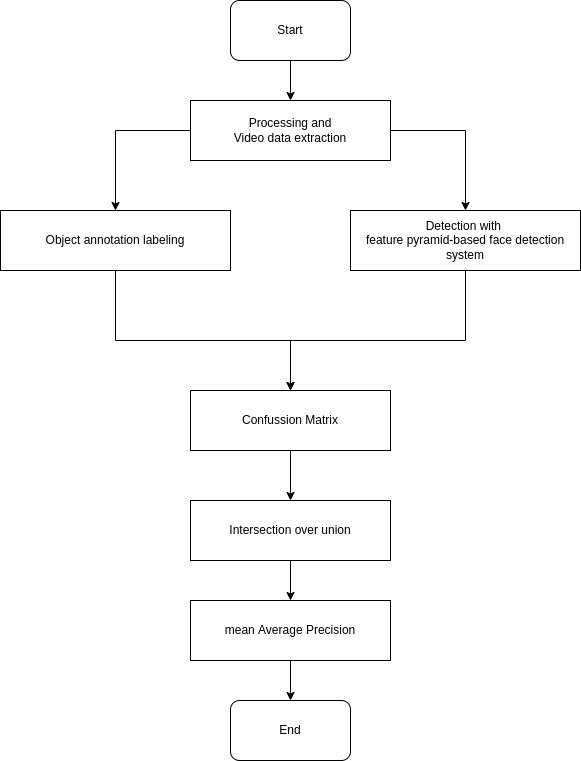
\includegraphics[width=0.4\textwidth]{gambar/blockdiagram.png}

  % Ubah sesuai dengan keterangan gambar yang diinginkan.
  \caption{Block diagram of this research}
  \label{fig:blockdiagram}
\end{figure}

The system design in this final project is designed to evaluate the performance of the pyramid network feature-based face detection system. Evaluation is done by
utilizing a face detection system that runs on a computer 
and video input obtained from previous research and used with permission from the author of \citep{nugrohoevalution2016}. 
Evaluation is done by comparing the mean Average Precision (mAP) on the results detection by the system used.

The process of evaluating a face detection system based on the pyramid network feature is shown in Figure \ref{fig:blockdiagram}.
Based on the flow chart in Figure \ref{fig:blockdiagram},
First process
what is done is processing and extracting video data. Purpose of video data processing and extraction
this is to get the frame of each video scenario.
The data frame obtained from the extraction is then given a label or annotation in the form of a ground-truth bounding box indicating where
the position of the face is in the video data.
The annotation process is carried out using open source open labeling tools.

Face detection system that
used in this study is a system that uses
feature-based object detection method pyramid network with two different backbones,
namely using mobilenet0.25 and resnet50 backbones.
Pyramid network feature-based face detection system will provide results
detection in the form of confidence, predicted bounding box and landmarks.
The results of face detection are then evaluated using a confusion matrix
and the Intersection over Union (IoU). These two values are used to form a precision-recall curve. The Average Precision (AP) value is obtained from the value under the curve, Next
these values are averaged so that the mean Average Precision (mAP) is obtained.

\subsection{Testing Scenario}
\label{subsec:skenariopengujian}

The purpose of the designed test scenario is to perform analysis
performance of the face detection model in a certain aspect.
In this study, five different scenarios were used
with various aspects. The data used are data from previous studies used with the permission of the author \citep{nugrohoevalution2016}.

The test scenarios obtained from the dataset are as follows:
\begin{enumerate}
  \item Testing Scenario Based on Data Collection Time

  Testing based on the time of data collection aims to find out
  effect of data retrieval time on computational performance and face detection results.
  Different time can describe different light conditions, Generally face detection system
  have difficulty when the light is very dark or the light is very bright. Based on this on
  In this scenario, data was collected during the day and at night to compare whether the system
  Pyramid network feature-based face detection got better results in one of these conditions, both
  conditions or worse in both conditions.

  In addition to light conditions, the data used is also regulated by various obstacles
  to find out specifically how accurate the face detection system based on the pyramid network feature is in easy, medium, or difficult obstacle conditions.
  The combination of obstacles provided is described as follows:
  \begin{itemize}
    \item Normal.
    \item Glasses.
    \item Mask.
    \item Hat.
    \item Hoodies.
    \item Glasses, masks.
    \item Glasses, hats.
    \item Glasses, hoodies.
    \item Masks, hats.
    \item Masks, hoodies.
    \item Hats, hoodies.
    \item Glasses, masks, hats.
    \item Glasses, masks, hoodies.
    \item Glasses, hats, hoodies.
    \item Masks, hats, hoodies.
    \item Glasses, masks, hats, hoodies.
    \item Sunglasses.
    \item Sunglasses, masks.
    \item Sunglasses, hats.
    \item Sunglasses, hoodies.
    \item Sunglasses, masks, hats.
    \item Sunglasses, masks, hoodies.
    \item Sunglasses, hats, hoodies.
    \item Sunglasses, masks, hats, hoodies.
  \end{itemize}
  \item Test Scenario Based on Number of Objects
  
  In the test scenario based on the number of objects, the aim is to find out
  the effect of the number of objects on the ability of the face detection system to detect faces.
  In this test, a camera above is used with a height of $260 cm$ and an elevation angle of $50^\circ$.
  The time of data collection was carried out during the day.
  There are ten conditions of the number of objects used,
  among others:

  \begin{itemize}
    \item Two people walking parallel.
    \item Two people walk hand in hand.
    \item Three people walking parallel
    \item Two people walk in parallel followed by one person walking alone behind him.
    \item One person walks alone followed by two people walking parallel behind him.
    \item Four people walk in parallel.
    \item Three people walk in parallel followed by one person walking alone behind him.
    \item One person walks alone followed by three people walking parallel behind him.
    \item One person walking alone followed by two people walking parallel and followed again by
    one person walking alone behind him.
    \item Two people walking parallel followed by two people walking parallel behind him.
  \end{itemize}

  \item Test Scenario Based on Object Velocity
  
  Testing based on the velocity of a moving object aiming
  to determine the effect of object velocity on the ability
  face detection system. In this test the data obtained are
  data during the day. There are three scenarios of object velocity conditions used,
  among others:

  \begin{itemize}
    \item An object moving at normal speed (average speed $0.68 m/s$).
    \item An object that is moving at a rather fast speed. (average speed $1.0 m/s$)
    \item An object that moves at a fast speed. (average speed $1.64 m/s$)
  \end{itemize}
  
  \item Test Scenarios with Addition of Artificial Light
  
  Testing with the addition of artificial lighting aims to determine the effect of
  light on the performance of face detection systems based on the pyramid network feature.
  The data obtained from this scenario is the data conditioned by the lighting.
  The artificial light used in this scenario is obtained from LED lamps for photography with
  lux size of 860 lumens and power of 9 watts. The hitch scenario in this test is in accordance with 
  scenario on Testing Scenario Based on Data Collection Time and the time of data collection is done at night with
  the condition of the camera that is above and the camera that is parallel to the face.
  
  \item Testing Scenario Based on Camera Angle
  
  Testing based on different camera angles aims
  to determine the effect of changing camera angles on
  the system's ability to detect faces. In this test,
  data collection during the day. There are five condition scenarios
  camera angle used, between
  other:

  \begin{itemize}
    \item Camera angle $30^\circ$
    \item Camera angle $40^\circ$
    \item Camera angle $50^\circ$
    \item Camera angle $60^\circ$
    \item Camera angle $70^\circ$
  \end{itemize}
  
\end{enumerate}


% \subsection{Lorem Ipsum}
% \label{subsec:loremipsum}

% \lipsum[11]

% % Contoh pembuatan tabel.
% \begin{table}
%   \caption{Contoh tabel sederhana}
%   \label{tab:tabelsederhana}
%   \centering
%   \begin{tabular}{lll}
%     \toprule
%     Heading1 & Heading2 & Heading3  \\
%     \midrule
%     One      & Two      & Three     \\
%     Four     & Five     & Six       \\
%     \bottomrule
%   \end{tabular}
% \end{table}

% % Contoh pembuatan potongan kode.
% \begin{lstlisting}[
%   language=C++,
%   caption={Program halo dunia.},
%   label={lst:halodunia}
% ]
% #include <iostream>

% int main() {
%     std::cout << "Halo Dunia!";
%     return 0;
% }
% \end{lstlisting}

% \lipsum[12]

% % Contoh pembuatan daftar.
% \begin{enumerate}
%   \item \lipsum[13][1-4]
%   \item \lipsum[13][5-8]
%   \item \lipsum[13][9-12]
% \end{enumerate}

% \lipsum[14-15]

\subsection{Object Labeling}
\label{subsec:pelabelanwajah}

Labeling or annotating objects is the process of providing information
in the form of class and position of the object to be detected.
From the frame obtained from the data extraction process, labeling is carried out
one by one to the face object so that the coordinates are obtained
ground-truth bounding box to be compared with the predicted bounding box.
Of the two types of existing bounding boxes, it will be
the value of the Intersection over Union (IoU) is obtained based on
comparison of the two bounding boxes.

The labeling process for bounding boxes is carried out one by one separately
manually on each frame that has a face object in it.
Information about the labels that have been created are then stored in the
TXT file format with the format: class-name-coordinate-x-point-top-left-coordinate-y-point-left-top-coordinate-x-point-bottom-right-coordinate-y-point-bottom-right.
From this stage, the TXT file was $27,093$ and the bounding box was $12,272$.

\subsection{Face Detection}
\label{subsec:pendeteksianwajah}

In this process, face detection is carried out using
programs that have been made previously and then carried out
changing parameters as well as adding code to suit
needs. In this study, two types of backbone were used.
on the feature pyramid network-based face detection model, namely mobilenet0.25
and Resnet50.
The output of the face detection process is confidence, class name
as well as the position of the bounding box of the faces detected by the system.
The three values obtained are the required values
on the performance analysis process of the method used.

A face detection system based on feature pyramid network requires an input image with a resolution
$640\times640$ that input will be processed by backbone to get a pyramidal hierarchy.
Each level that forms this pyramidal hierarchy is obtained from each of the residual network outputs
if on Resnet50. If on mobilenet0.25 each pyramidal hierarchy is obtained from output depthwise separable convolutions
This pyramidal hierarchy with resolution that has been scaled with different levels
will be processed using the feature pyramid network architecture.

The output of feature pyramid network is feature maps with different sizes
(according to the number of levels obtained from the pyramidal hierarchy) with the number of channels $256$. Next each
this output will be processed by context module. Context module aims to strengthen context modeling capacity
so that the feature maps obtained is more accurate. In the context module the deformable convolutional and lateral connection processes are carried out
and the output will be the same size as the input but with a stronger context modeling capacity.

Then each feature maps will be processed by multi-task loss to get bounding-box, confidence and landmarks.
For negative anchor conditions, the feature pyramid network-based face detection system will only process for classification, and will not issue
other outputs such as bounding-box, confidence and landmarks \citep{deng2019retinaface}.
